\chapter{Measurement of the inclusive $t\bar{t}+\gamma$ cross-section}\label{chap-crosssection}

\section{Signal Definition and Background Processes}

\subsection{Signal definition}

\begin{figure} \label{fig-signalphotonplot}
\begin{center}
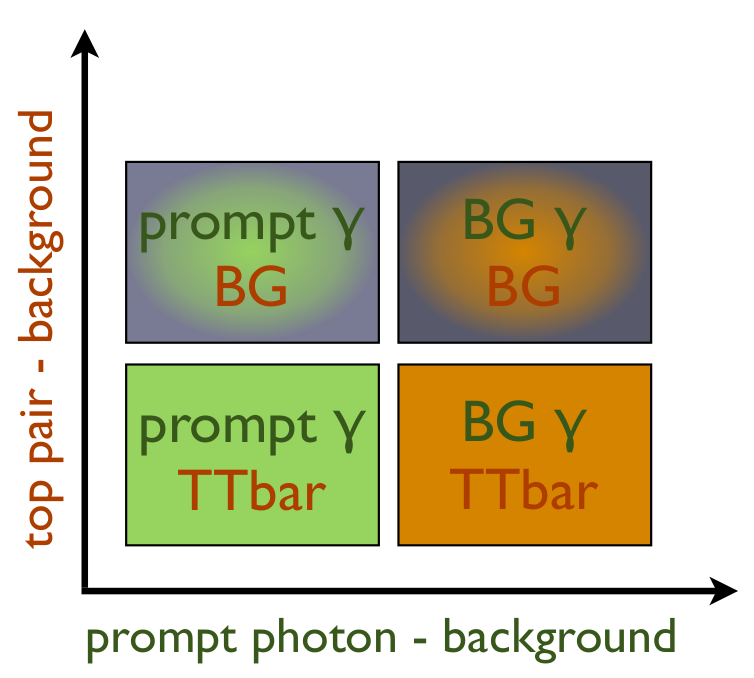
\includegraphics[scale=0.33]{Figures/SignalPhotonPlot.png}
\caption{Graphic representation of the signal and background definitions \cite{MishaSignalDefinition}.}
\end{center}
\end{figure}

\subsection{Background processes}

\begin{figure}
\begin{center}
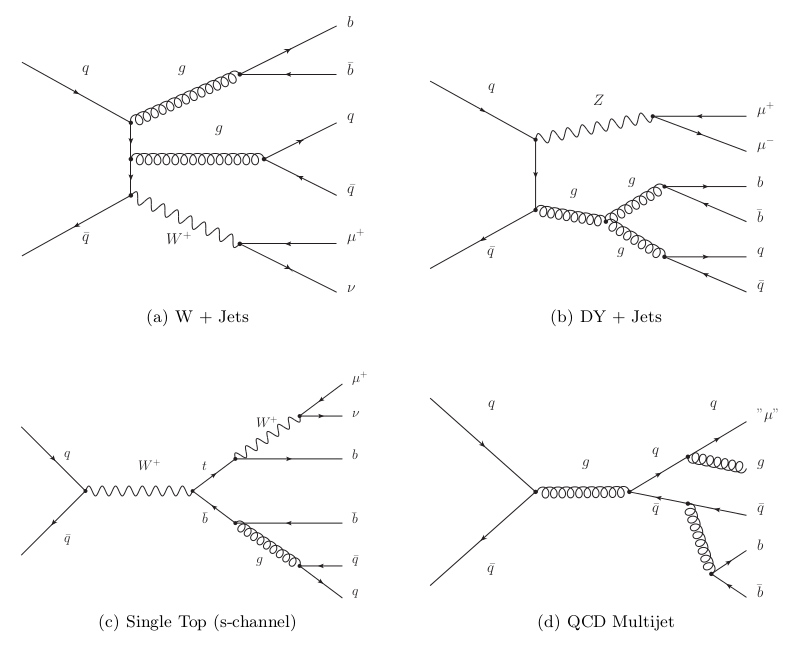
\includegraphics[width=\textwidth]{Figures/BackgroundDiagrams.png}
\caption{Examples of Feynman graphs of the considered $t\bar{t}$ backgrounds. QCD showering is necessary in all cases to obtain the required jet multiplicity \cite{ttgammabackgroundestimation}.}
\end{center}
\end{figure}

\begin{figure}\label{fig-AnalysisFlowChart}
\begin{center}
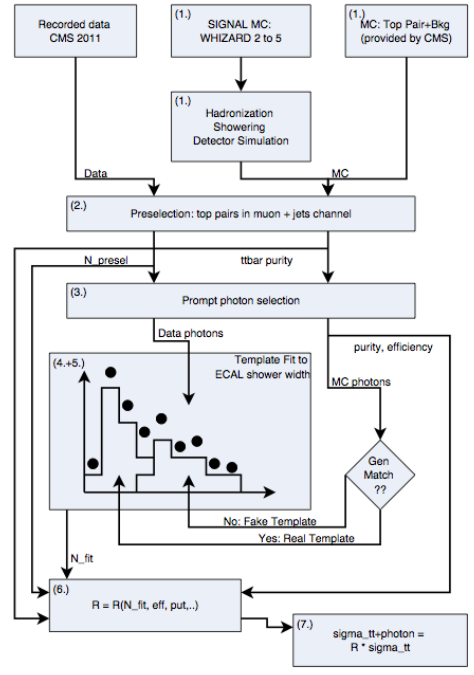
\includegraphics[width=0.75\textwidth]{Figures/AnalysisFlowChart.png}
\caption{Flow chart showing each stage of the analysis. The box numbers represent the outlined
analysis steps.}
\end{center}
\end{figure}

\subsection{Backgrounds of photon signature}

\begin{figure} \label{fig-BackgroundISR}
\begin{center}
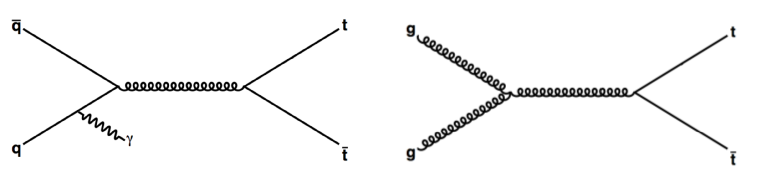
\includegraphics[width=\textwidth]{Figures/BackgroundISR.png}
\caption{Background of photon identification: Initial state radiation (ISR). Left: Quark fusion. Right: Gluon fusion does not give rise to ISR (based on \cite{photonbackgrounds}).}
\end{center}
\end{figure}


\begin{figure} \label{fig-BackgroundFSR}
\begin{center}
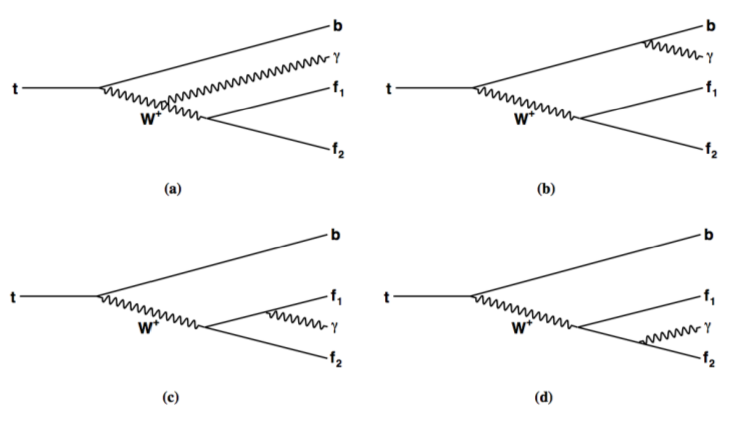
\includegraphics[width=\textwidth]{Figures/BackgroundFSR.png}
\caption{Background of photon identification: Final state radiation (FSR). All charged particles in the top-pair decay tree contribute to FSR \cite{photonbackgrounds}.}
\end{center}
\end{figure}

\section{$t\bar{t}+\gamma$ Signal Simulation}

WHIZARD

then

MADGRAPH

Factorised matrix element 

\section{Phase Space Overlap Removal} \label{sec-PhaseSpaceOverlapRemoval}

Events of the $t\bar{t}+\gamma$ process lie within a small region of $t\bar{t}$ phase space, and thus our signal sample events are expected to overlap with TTJets events in the case where a hard photon is radiated by initial state quarks, top quarks, b quarks, W and its decay products: electrons, muons, and their corresponding neutrino. In order to prevent the double counting of events we apply an overlap removal procedure to remove such events from our TTJets samples. In order for an event to be considered as overlapping with TTGamma, an event has to have at least one generator-level photon with the following properties:

\begin{itemize}
	\item p$_T(\gamma) > 13$ GeV
	\item $|\eta| < 3.0$
	\item Only gluons, bosons, or leptons are in the parents list. This ensures that photons from $\pi^0$ decays are not considered as signal
	\item $\Delta R(\gamma, other) > 0.2$ where other particles include leptons, b quarks and final state particles (hadrons, charged leptons, photons) with transverse momenta above $5 \GeV$.
\end{itemize}

The last cut is implemented in order to suppress photons from showers. In such cases the information from the parent particle will show that a photon is radiated by an electron, however the photon may be collinear with it. In particular in TTJets di-lepton events, such as described in this analysis, where a considerable fraction of the reconstructed photons comes from electrons radiating photons.

 Similarly, we also observe an overlap between Z+Jets and ZGamma processes, and between W+Jets and WGamma samples, for the same reasons as described above. The phase space overlap removal procedure is applied on Z+Jets and W+Jets samples to remove events containing generator-level photons. Events containing generated photons are removed in the case in which they are from initial state radiation (emitted from the colliding partons) or final state radiation (emitted from W or Z bosons or their decay products), since these are already included in the WGamma and ZGamma simulations. The overlap removal procedure removes approximately one percent of the events in the W+Jets sample, and approximately three to four percent of the events from the TTJets and Z+Jets samples.

\begin{figure} \label{fig-photonphasespace}
\begin{center}
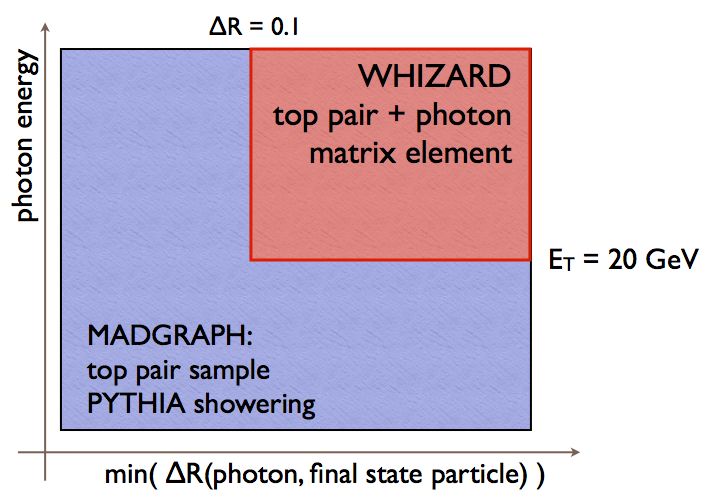
\includegraphics[scale=0.5]{Figures/photonphasespace.png}
\caption{}
\end{center}
\end{figure}

\section{Measurement of the cross-section ratio $R = \sigma_{t\bar{t}+\gamma}/\sigma_{t\bar{t}}$}

A common form of cross-section calculation for a ``counting'' analysis can be written as

\begin{equation} \label{eqn-CountingXsect}
\sigma = \frac{N_{signal}}{\lumi \epsilon A}
\end{equation}

where $N_{signal}$ is the number of signal events found in data passing the full event selection requirements, $\lumi$ is the integrated luminosity of the data, $A$ is the signal acceptance, defined as the fraction of signal events that fall into the region of phase-space that is chosen for our event selection, and $\epsilon$ is the efficiency of correctly selecting a signal event (the fraction of signal events passing event selection after acceptance cuts are implemented). The number of signal events, $N_{signal}$, must be modified to account for the presence of background events in our data, and thus becomes the number of observed events minus the number of background events, $N_{observed} - N_{background}$, where the number of background events is estimated in a different manner. 

Due to the nature of the analysis, event selection is performed in two separate steps (see Section \ref{chap-EventSelection}); di-leptonic top pair selection and photon selection. This feature changes the way in which we must compute the cross-section in Equation \ref{eqn-CountingXsect}. The changed cross-section is written as

\begin{equation}
\sigma_{t\bar{t}+\gamma} = \frac{N_{signal}}{\lumi \epsilon_{top} A_{top} \epsilon_{\gamma} A_{\gamma}}
\end{equation}

where $\epsilon_{top}$ and $A_{top}$ are the efficiency and acceptance of top selection for our signal top pair events. Thus, $\epsilon_{\gamma}$ and $A_{\gamma}$ are the efficiency and acceptance of the photon selection, introduced after the top quark pair event selection. Here we consider our signal as a top quark pair, decaying to leptons and b-jets, plus a prompt radiatied photon as our signal. We take the number of obvserved, $N_{signal}$, as the number of events counted from data after top pair and photon selections have been applied.

In order to simplify the calculation, we are able to take the ratio of the $t\bar{t}+\gamma$ cross-section to the $t\bar{t}$ cross-section, as previously measured by the CMS experiment \cite{ttbarXsectiondilepton}. In doing this, we simplfy the treatment of systematic uncertainties and cancel shared terms from each measurement, such as luminosity. The new ratio is calculated using the following equation

\begin{equation}
R = \frac{\sigma_{t\bar{t}+\gamma}}{\sigma_{t\bar{t}}} = \frac{N_{signal}}{\epsilon^{t\bar{t}+\gamma}_{top} A^{t\bar{t}+\gamma}_{top} 
\epsilon^{t\bar{t}+\gamma}_{\gamma} A^{t\bar{t}+\gamma}_{\gamma}}} \cdot \frac{\epsilon^{t\bar{t}}_{top} A^{t\bar{t}}_{top}}{N_{t\bar{t}}}
\end{equation}

We now introduce a second term into the cross-section calculation which includes three new variables that stem from the $t\bar{t}$ inclusive cross-section: where $\epsilon^{t\bar{t}}_{top}$ and $A^{t\bar{t}}_{top}}$ $N_{t\bar{t}}$ are the efficiency and acceptance of the $t\bar{t}$ process, and $N_{t\bar{t}}$ is the number of top pair events passing the full top selection, prior to the photon selection. The efficiencies for both top pair selection and top pair with a photon selection is very similar due to the ordering of the event selection - the selection of leptons, jets, b-jets, and MET are the same in each scenario. As the acceptance calculation depends on individual samples generator cuts and even selection, we must calculate this variable separately for each stage of the selection process. By taking the ratio of each cross-section we cancel out the luminosity parameter.

The prominent feature of this analysis is the addition of a radiated photon from one of the decay products of a di-leptonic $t\bar{t}$ decay. In order to correctly measure the number of signal $t\bar{t}+\gamma$ events we must make sure that we have correctly identified our signal events. Even though an object may pass the full photon ID selection requirements, it may not be our signal photon. Electrons and jets are likely to pass photon ID selection and be recorded as real signal photons, thus we must remove these `fakes' from our signal events.

For jets that pass the photon ID requirements and are thus misidentified, we must note that they do not contain a genuine photon. Electrons that have been misidentified as photons are more difficult to remove as they hold the same properties as a photon, including isolated electromagnetic shower etc. Electrons differ from our signal photons because of the addition of a charged track pointing in the direction of the energy deposit. As a result, we treat each source of `fakes' in a different manner, described in Section \ref{}.   



\section{Number of top pair events}



\section{Photon Purity Estimation} \label{sec-PhotonPurityEstimation}

We define the photon purity, $\pi$, as the number of photons that are prompt and pass the photon ID selection over the total number of photon candidates. Prompt photons are created in the hard-scattering process and are emitted from the high-$p_T$ hard-scattering particles. The main sources of non-prompt photons comes from charged particles interacting with the detector material and from quark hadronisation, and are generally not isolated and have a low $p_T$. We also obtain a source of photons from $\pi^0$ decays, whereby two very collinear photons are produced. 

One method to find the photon purity is through simulation, where we have access to information of all the particles simulated by the MC event generator. We match reconstructed photons to generator photons by using information of their mother particles in order to determine the origin of the photons. From this, we can divide our events into three categories based on the event generator matching to a reconstructed photon. 

\begin{itemize}
	\item Signal: reconstructed photon is matched to a generated photon
	\item Misidentified electron: reconstructed photon is matched to a generated electron
	\item Misidentified jet: photon is not matched to either a generated photon or electron
\end{itemize}

In order to find if our photon is prompt (signal), we use our matching process to find a generator-level photon that matches its properties. We use the transverse momentum along with the $\eta$ and $\phi$ coordinates of the reconstructed and generator-level photon to implement a $p_T$ and $\Delta R$ requirement on the matching process. Events are iterated over in the order in which they were created by the generator, and if we find the $\Delta R$ between the reconstructed photon and generated photon is \textbf{less than 0.2} and $|p^{reco}_T - p^{gen}_T|/p^{gen}_T$ is \textbf{less than 1.0} then we consider it a match and stop the iteration process. The parentage of the matched photon is then inspected to verify its origin, such that if it descends from a quark, gluon, charged lepton, or boson then we determine it to be prompt. We must, however, also verify that the photon is isolated. A photon maybe produced in the hard-scattering process, however we may observe hadronisation and showering in close by, such that our signal photon will not be isolated. In order to ensure that these photons are not lost to the nearby non-signal activity, we must introduce additional selection cuts to differentiate between our prompt signal photons and non-isolated photons.  

\begin{itemize}
	\item $\left(p_T^{reco} - p_T^{gen}\right)/p_T^{gen} < 0.1$
	\item $\Delta R ( \gamma^{gen}, other ) > 0.2$ where other particles include leptons, photons and final state
particles (hadrons, leptons, photons) with transverse momenta above 5 GeV
	\item $|\Delta\eta ( \gamma^{reco}, \gamma^{gen} )| < 0.005$
	\item $\Delta R ( \gamma^{reco}, \gamma^{gen} ) < 0.01$
\end{itemize}

The listed additional cuts help to select photons that are well isolated and do not have any undesired activity nearby.

As described above, electrons leave a very similar trace to photons as it showers within the electromagnetic calorimeter, except for an additional charged track pointing towards the energy deposit. We implement specific selection criteria in order to minimise the fake-rate of electrons misidentified as photons within the event selection. However, it is observed that a large number of electrons still pass photon selection requirements and are recorded as signal. We thus include a criteria to find well isolated generator-level electrons in the same manner as for photons, however in this scenario we consider electrons from W and Z decays only. The cuts are shown below.

\begin{itemize}
	\item $\left( p_T^{reco} - p_T^{gen} \right) /p_T^{gen} < 0.1$
	\item $\Delta R ( e, other ) > 0.2$ where other particles include leptons, photons and final state
		  particles (hadrons, leptons, photons) with transverse momenta above 5 GeV
	\item $ \Delta\eta ( \gamma^{reco}, e )| < 0.005$
	\item $\Delta R ( \gamma^{reco}, e ) < 0.04$
\end{itemize}

The cuts have been cross-checked with the di-leponic $t\bar{t}$ sample as it contains a significant amount of electrons identified as photons.

All reconstructed photons that pass the cuts described previously and is matched with a generator-level photon is then defined as a real photon. If it is instead matched to a generator-level electron it is then defined as a misidentified electron. Any other event that is not matched to a generator-level electron or photon is then classified as a misidentified jet.

As the photon purity directly affects the cross-section ratio measurement, we do not want to reply explicitly on simulation, and therefore it would be preferable to compute the photon purity via a data-driven method. We make use of the fact that our signal photon, whether a real signal photon or misidentified electron, are isolated objects, while misidentified jets and non-prompt photons close to or within a jet. 

%  We use super cluster removed charged hadron isolation as discriminating variable. Then
% the template shape fit is performed to find the fraction of prompt photons. The template fit
% provides an estimate of the fraction of events originating from real photons or misidentified
% electrons

\cite{PhysRevD.89.092005}

\section{Number of signal events in data} \label{sec-SigEventsData}

\section{Signal Acceptance Calculation} \label{subsec-SignalAcceptanceCalculation}

Acceptance calculation for this analysis differs from usual inclusive cross section measurements because we measure ratio of cross sections. The event selection is chosen to make use of this fact: two steps (top selection and photon selection) are done sequentially. For the inclusive $t\bar{t}$ process, we start with number of generated events (within some fiducial phase space) and count how many events are left after top event selection. The acceptance times efficiency is defined for the $t\bar{t}$ top selection as:

\begin{equation}
	\epsilon^{t\bar{t}}_{top} \cdot A^{t\bar{t}}_{top} = \frac{N_{t\bar{t}.preselection}}{N_{t\bar{t}.generated}} 
\end{equation}

This gives the acceptance times efficiency of the inclusive $t\bar{t}$ process to be $\epsilon^{t\bar{t}}_{top} \cdot A^{t\bar{t}}_{top} =   \pm  (stat.)$ in the di-muon channel, $\epsilon^{t\bar{t}}_{top} \cdot A^{t\bar{t}}_{top} =  \pm  (stat.)$ in the di-electron channel, and $\epsilon^{t\bar{t}}_{top} \cdot A^{t\bar{t}}_{top} =  \pm  (stat.)$ in the mixed final state.

The same can be done for the $t\bar{t}+\gamma$ (signal sample). To get the acceptance times efficiency we have to divide the number of events passing top selection by the total number of events considered. However, in this case we have to choose what we take as the denominator. The signal $t\bar{t}+\gamma$ sample is inclusive, but theoretical calculations for the cross section are done for final states with 1 and 2 leptons \cite{QCDCorrectionsttgamma2011}. To make comparison with theory easier we consider the fiducial space for signal when 1 or 2 leptons are present. The $t\bar{t}+\gamma$ acceptance times efficiency of the top selection is defined for the signal samples with 1 or 2 leptons as:

\begin{equation}
	\epsilon^{t\bar{t}+\gamma}_{top} \cdot A^{t\bar{t}+\gamma}_{top} = \frac{N_{t\bar{t}+\gamma.preselection(1lor2l)}}{N_{t\bar{t}+\gamma.generated(1lor2l)}} 
\end{equation}

Giving the acceptance times efficiency of the inclusive $t\bar{t}+\gamma$ process to be $\epsilon^{t\bar{t}+\gamma}_{top} \cdot A^{t\bar{t}+\gamma}_{top} =   \pm  (stat.)$ in the di-muon channel, $\epsilon^{t\bar{t}+\gamma}_{top} \cdot A^{t\bar{t}+\gamma}_{top} =  \pm  (stat.)$ in the di-electron channel, and $\epsilon^{t\bar{t}+\gamma}_{top} \cdot A^{t\bar{t}+\gamma}_{top} =  \pm  (stat.)$ in the mixed final state.

The acceptance and efficiency for the $t\bar{t}+\gamma$ sample includes a term for photon selection. This is found based on the ratio of the number of events in $t\bar{t}+\gamma$ passing photon selection and the reconstructed photon matched to a generated photon over the number of events passing the top selection. The $t\bar{t}+\gamma$ photon selection acceptance times efficiency is defined as

\begin{equation}
	\epsilon^{t\bar{t}+\gamma}_{\gamma} \cdot A^{t\bar{t}+\gamma}_{\gamma} = \frac{N_{t\bar{t}+\gamma.photonselection(1lor2l)}}{N_{t\bar{t}+\gamma.preselection(1lor2l)}} 
\end{equation}

Thus, yields of the acceptance times efficiency of the inclusive $t\bar{t}+\gamma$ process to be $\epsilon^{t\bar{t}+\gamma}_{\gamma} \cdot A^{t\bar{t}+\gamma}_{\gamma} =   \pm  (stat.)$ in the di-muon channel, $\epsilon^{t\bar{t}+\gamma}_{\gamma} \cdot A^{t\bar{t}+\gamma}_{\gamma} =  \pm  (stat.)$ in the di-electron channel, and $\epsilon^{t\bar{t}+\gamma}_{\gamma} \cdot A^{t\bar{t}+\gamma}_{\gamma} =  \pm  (stat.)$ in the mixed final state.

The calculation of signal acceptance explained above is done for the sake of comparison with theoretical prediction. The biggest difference in the generated phase space and analysis selection is the transverse energy cut on the photon (13 GeV in generated sample and 25 GeV in analysis). We are measuring the value for the higher $E_T$ cut on the photon and using the efficiencies to extrapolate back to the full generated phase space. In order to avoid this propagation of the result into the larger phase space we also quote the \emph{visible cross section ratio}, where the cross section is measured in the fiducial region with generated photons having transverse energy of at least 25 GeV and $| \eta | < 1.4442$. For the visible cross section ratio, the photon selection term includes only the photon reconstruction efficiency because, by definition, we are considering events where generator photon passes analysis level $p_T$ and $\eta$ cuts.

The visible top selection efficiency in $t\bar{t}+\gamma$ is taken to be the ratio of the number of $t\bar{t}+\gamma$ events passing the preselection (with a generated photon having $p_T > 25$ GeV and $| \eta | < 1.4442)$

\begin{equation}
	\epsilon^{t\bar{t}+\gamma Vis}_{top} = \frac{N_{t\bar{t}+\gamma.preselection(1lor2l)}\left( p_T(\gamma_{gen}) > 25 GeV, |\eta(\gamma^{gen})| < 1.4442 \right)}{N_{t\bar{t}+\gamma.generated(1lor2l)}\left( p_T(\gamma_{gen}) > 25 GeV, |\eta(\gamma^{gen})| < 1.4442 \right)} 
\end{equation}

The $t\bar{t}+\gamma$ visible photon selection efficiency is calculated as the ratio of $t\bar{t}+\gamma$ events passing to photon selection with a reconstructed photon matched to a generated photon over the number of events passing top selection and with an isolated generator level photon passing the $p_T > 25$ GeV and $| \eta | < 1.4442$ cuts used in the photon selection.

\begin{equation}
	\epsilon^{t\bar{t}+\gamma Vis}_{\gamma} = \frac{N_{t\bar{t}+\gamma.photonselection(1lor2l)}\left( p_T(\gamma_{gen}) > 25 GeV, |\eta(\gamma^{gen})| < 1.4442 \right)}{N_{t\bar{t}+\gamma.preselection(1lor2l)}\left( p_T(\gamma_{gen}) > 25 GeV, |\eta(\gamma^{gen})| < 1.4442 \right)} 
\end{equation}

The visible top selection efficiency is found to be $\epsilon^{t\bar{t}+\gamma Vis}_{top} = 0.0712 \pm 0.0005$, $\epsilon^{t\bar{t}+\gamma Vis}_{\gamma} = 0.0928 \pm 0.0006$, and $\epsilon^{t\bar{t}+\gamma Vis}_{\gamma}$ in the di-muon, di-electron and mixed channels, respectively. The value of the visible photon selection efficiency is found to be $\epsilon^{t\bar{t}+\gamma Vis}_{\gamma} = 0.287 \pm 0.004 ( stat.)$ for the di-muon final state, $\epsilon^{t\bar{t}+\gamma Vis}_{\gamma} = 0.286 ± 0.004 (stat.)$ for the di-electron channel, and $\epsilon^{t\bar{t}+\gamma Vis}_{\gamma} = 0.287 \pm 0.004 ( stat.)$ for the mixed final state.